\chapter[Introduction]{Introduction}
\label{Chap:Introduction}

\section{Topic Definition}
In recent years, growth of the Internet of Things (IoT) has led to an unprecedented increase in the number of internet-connected devices, with estimates suggesting that there will be over 75 billion IoT devices by 2025 \cite{Alam2018}. However, this growth has brought to attention the importance of network security in embedded systems, especially where sensitive data is handled. Cyber-attacks targeting IoT devices have become more sophisticated and frequent, with the number of IoT attacks increasing by 300\% in 2019 alone \cite{Michael2019}. The financial impact of these attacks is staggering, with the annual cost of data breaches speculated to reach \$10.5 trillion by 2025 \cite{Morgan2020}. 

Trends in the IoT space such as edge computing, 5G networks, and artificial intelligence (AI) are sky-rocketing the demand for highly-performant processing solutions \cite{Nuttall2018} while traditional software-based security approaches often struggle to keep up with the real-time requirements and resource constraints of IoT devices \cite{Frustaci2018}. Frustaci et al. \cite{Frustaci2018} highlight the limited memory, processing power, and energy resources of IoT devices make it challenging to implement strong security measures using software alone without compromising performance and battery life. This is where FPGAs can offer a solution. By leveraging the flexibility of FPGAs, it is possible to create an optomised and dedicated network security solution.

This thesis proposes the development of a RISC-V softcore processor specifically designed for network security in embedded IoT applications. The use of RISC-V has several advantages over other contemporary architectures. For one, it is an open-source instruction set architecture that is concise, modular, and extensible \cite{Patterson2017}. Its open nature allows for customization of the processor design to meet specific requirements, while its modular design enables the addition of custom instructions and extensions to emphasise security-related tasks \cite{Waterman2016}. With this, the project aims to show how a dedicated solution can mitigate potential threats at the hardware level.
\clearpage

\subsection{Aims}
The aims for a successful FPGA-based edge device are as follows:
\begin{enumerate}
    \item Increase network security.
    \item Minimise processing latency.
    \item Maximise power efficiency.
    \item Minimise Resource Utilisation.
\end{enumerate}

\subsection{Key Performance Indicators}
The previous aims will then be evaluated against the following criteria:
\begin{enumerate}
    \item\textbf{Network Security:}\newline Penetration testing and vulnerability assessments will be conducted against a chosen network security method, see section ~\ref{sec:Project Overview}. The number and severity of detected security threats will gauge the effectiveness of the security features. The subsequent key performance indicators also contribute to overall network security.
    \item\textbf{Processing Latency:}\newline packet processing time will be measured under various idle, average and peak network conditions. This will involve testing the system with different packet sizes and security features enabled to assess the impact on latency. The latency results will also be compared with similar security solutions to benchmark the performance of the FPGA-based processor.
    \item\textbf{Power Efficiency:}\newline Power consumption will be measured during idle, average, and peak loads. The energy efficiency ratio (performance per watt) will be calculated to provide a standardized metric for comparison. The power efficiency of the system will be compared with other FPGA-based and software-based solutions to assess its relative performance. Also, a thermal camera will be used to visualise the heat radiation from the FPGA. There is also the possibility of using the integrated temperature sensor on the Arty S7 Board \cite{ArtyS7RefManual} for plots.
    \item\textbf{Resource Utilisation:}\newline Resource utilization will be evaluated by measuring the counts of FPGA resources in the FPGA design software, such as look-up tables (LUTs), flip-flops and block RAM (BRAM). Memory and CPU utilization on the target IoT devices will also be observed to ensure the system does not overburden the limited resources available.
\end{enumerate}
\clearpage

\section{Project Overview}
\label{sec:Project Overview}
This section will now pertain to the complete hardware and software stack of of the proposed solution. A high-level overview of which can be seen in figure \ref{Fig:1}.

\begin{figure}[h]
    \begin{center}
    \caption{High-Level Network Overview}
    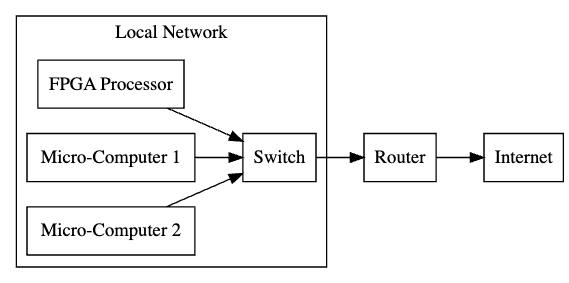
\includegraphics[width=1.0\textwidth]{./Figures/Network_Overview.png}
    \label{Fig:1}
    \end{center}
\end{figure}

Here, the local network refers to the arrangement of the edge devices in the network (left-hand side). It consists of the project's primary focus, the RISC-V softcore processor as well as two microcomputers which will be implemented as Raspberry Pis, (RPis). On the right hand side is the router which will interface the local network with the external internet structure, allowing packets to be received externally.

\subsection{FPGA Processor}
The FPGA will be running a real-time operating system, Zephyr. Zephyr has support for multicore designs as well as support for many types of peripherals and networking services. Functionality will be split across two cores as seen in figure \ref{Fig:2}. Core 0, will be the main core which will handle task-dispatching as well as peripheral interfacing (VGA, GPIO \etc). Like Core 1, which will handle the networking stack, it has access to a unified, shared memory block allowing it to subsequently access the processed packets. As the project progresses, the resource allocation for each core will be adjusted exclusively to their requirements.
\begin{figure}[h]
    \begin{center}
    \caption{High-Level FPGA Architecture Overview}
    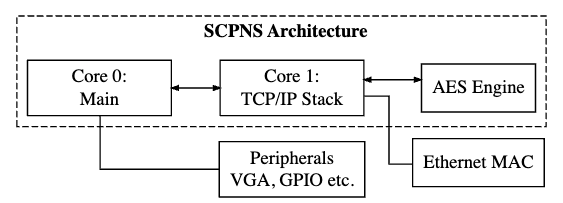
\includegraphics[width=1.0\textwidth]{./Figures/FPGA_Architecture_High_Level.png}
    \label{Fig:2}
    \end{center}
\end{figure}
\subsection{Microcomputers}
Basic software containers, deployed via Kubernetes, will run on the Microcomputers. These images will contain established libraries that provide TCP/IP stack interfacing as well as the ability to send/receive packets.
\subsection{Switch}
It has not been decided yet which switch will be used. Furthermore, communication protocols for the chosen commercial switch will need to be researched.
\subsection{Router}
It has not been decided yet which router will be used.
\subsection{Chosen Network Security Method}
To emphasise the network security aspect of the project, an additional layer of network security will be designed and implemented. It has not yet been decided which network security method will be used. Here, a custom hardware component will be designed that implements a typical network security method such as an accelerated cryptographic processor or a firewall that filters packets. The possible options are elaborated on in \ref{subsection:Network Security Methods}
\clearpage